\chapter{Das Hadoop Ecosystem}
Im Laufe der Jahre hat sich um den Kern von Hadoop ein reichhaltiges Ökosystem an weiteren Projekten gebildet (das Hadoop Ecosystem). Diese erweitern die Funktionalitäten des Kerns, oder ersetzen gar ganze Komponenten durch alternative Implementierungen. Hadoop ist so modular konzipiert, dass dies problemlos möglich ist. Das Ecosystem lässt sich grob in vier Kategorien aufteilen: Datenspeicherung, Verwaltung~/~Konfiguration, Datentransfer und Datenverarbeitung (vgl. Abb. \ref{fig:ecosys}). Ausgesuchte Komponenten werden in den nächsten Abschnitten kurz vorgestellt.

\begin{figure}[ht]
    \centering
    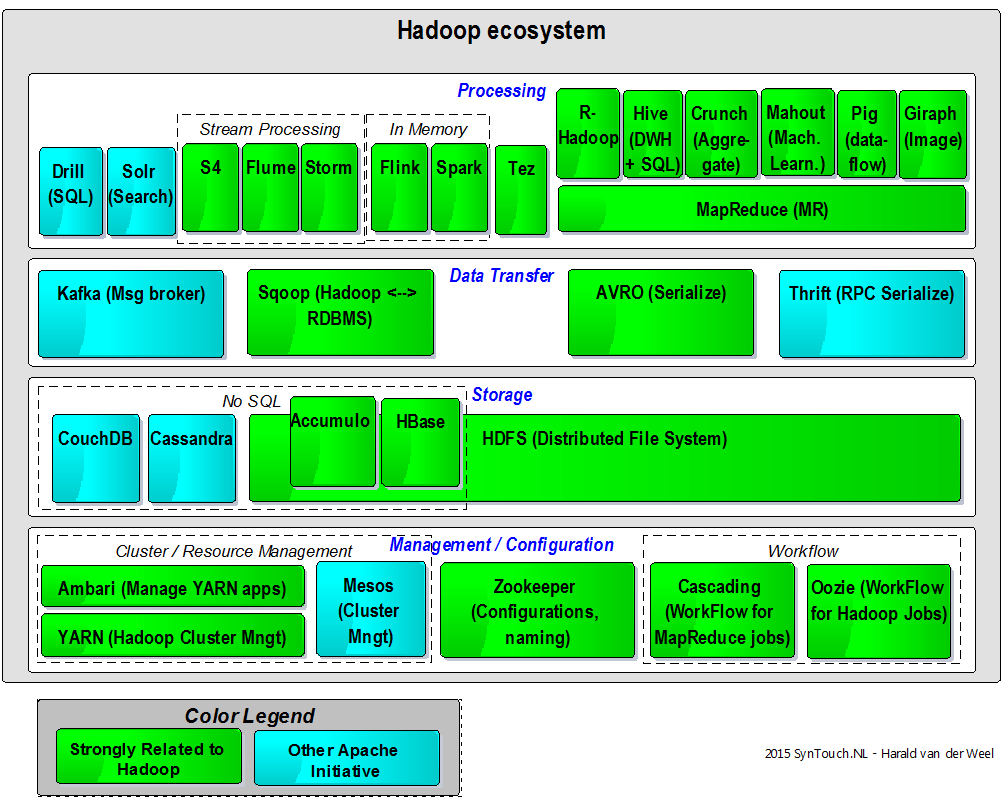
\includegraphics[width=\textwidth]{Hadoop_ecosystem_overview}
    \caption[Komponenten des Hadoop Ecosystems]{Komponenten des Hadoop Ecosystems\parencite{van_der_weel_hadoop_2015}}
    \label{fig:ecosys}
\end{figure}

\section{Datenhaltung}
\subsection{HDFS}
Das HDFS ist Hadoops mitgeliefertes Dateisystem für die verteilte Speicherung und den parallelen Zugriff auf Daten im Gigabyte- bis Terabyte-Bereich (siehe Kapitel \ref{chap:fund sec:core sub:hdfs}). Dabei stehen hohe Durchsatzraten und Verfügbarkeit im Vordergrund. Echtzeit-Zugriffe auf Daten im Millisekunden-Bereich sind nicht möglich. An Dateien kann außerdem zwar angehängt, aber nicht an beliebigen Stellen etwas eingefügt werden \parencite[vgl.][Kapitel 3]{white_hadoop_2015}. Für solche Anwendungsfälle kann Apache HBase verwendet werden. 
\subsection{HBase}
Apache HBase\footnote{https://hbase.apache.org/} ist eine nichtrelationale, verteilte Datenbank, die auf Hadoop und dem HDFS aufbaut. HBase bietet beliebige Lese- und Schreibzugriffe in Echtzeit auf Tabellen mit Milliarden von Zeilen und Millionen von Spalten. Datensätze werden in \textit{ColumnFamilies} und \textit{Columns} gespeichert, wobei beliebig Spalten hinzugefügt oder weggelassen werden können. HBase speichert solche dünnbesetzten Tabellen sehr effizient, da ein leerer Wert, ein \textit{null}, anders als bei relationalen Datenbanken keinen Festplattenspeicher belegt \parencite[vgl.][Abschnitt 21]{hbase_team_apache_2022}.  

\section{Cluster-Verwaltung / -Konfiguration}
\subsection{YARN}
YARN ist Hadoops Ressourcen-Manager und Job-Tracker (siehe Kapitel \ref{chap:fund sec:core sub:yarn}). Will eine Anwendung auf einem Hadoop Cluster laufen, fordert sie über YARNs API Ressourcen wie Prozessorkerne und Arbeitsspeicher in Form von \textit{Containern} an. YARN stellt diese auf ausgesuchten Nodes im Cluster bereit und abstrahiert den Aspekt der Verteilung. YARN übernimmt außerdem die Abarbeitung von Jobs durch konfigurierbare Warteschlangen. Durch YARN wird es möglich, Applikationen auf einem Hadoop Cluster verteilt laufen zu lassen, die nicht das MapReduce Framework benutzen.\parencite[vgl.][YARN $\rightarrow$ Architecture]{noauthor_apache_nodate}
\subsection{Oozie}
Apache Oozie\footnote{https://oozie.apache.org/} dient der Ablaufsteuerung von Hadoop Jobs. Durch Nutzung einer auf XML basierenden \textit{Process Definition Language}\footnote{https://oozie.apache.org/docs/5.2.1/DG\_Overview.html} werden Abhängigkeiten zwischen Hadoop Jobs modelliert, zum Beispiel wenn Job B Daten benötigt, die von Job A generiert werden. Oozie sorgt dafür, dass ein so definierter \textit{Oozie Workflow} sequenziell korrekt abgearbeitet wird. Mit \textit{Oozie Coordinator} kann man außerdem Auslösekriterien für Workflows definieren, wie eine Tageszeit oder die Verfügbarkeit eines neuen Datensatzes. 
\subsection{ZooKeeper}
Apache ZooKeeper\footnote{https://zookeeper.apache.org/} ist ein Service zur zentralen Verwaltung und Synchronisation kleiner Dateien (< 1 MB; Konfigurationsdateien) über einem Cluster. Anwendungen verwenden ZooKeeper für unterschiedliche Aufgaben: HBase überwacht mittels ZooKeeper die Verfügbarkeit seiner RegionServer\footnote{vgl. https://blog.cloudera.com/what-are-hbase-znodes/}. Das HDFS kann im \textit{High Availability Mode} einen sekundären NameNode bereithalten, welcher ohne signifikante Ausfallzeit den NameNode ersetzen kann, sollte dieser ausfallen. Dieser \textit{Automatic Failover} wird von ZooKeeper angestoßen\footnote{https://hadoop.apache.org/docs/stable/hadoop-project-dist/hadoop-hdfs/HDFSHighAvailabilityWithQJM.html}.
\subsection{Ambari}
Apache Ambari\footnote{https://ambari.apache.org/} ermöglicht die Provisionierung, Verwaltung und Überwachung von Apache Hadoop Clustern mittels einer Reihe von übersichtlichen Web-Dashboards. Es wurde zum Teil bereits in Kapitel \ref{chap:handson sec:ambari} benutzt. Mit Ambari kann man eine Vielzahl von Hadoop Services im Cluster installieren, konfigurieren und den Zustand des Clusters anhand diverser Metriken überwachen.

\section{Datentransfer}
\subsection{Sqoop}
Apache Sqoop\footnote{https://sqoop.apache.org/} war ein Top-Level Projekt von Apache, bis es im Juni 2021 eingestellt wurde. Es ist noch zum Download verfügbar und kommerzielle Anbieter wie Cloudera bieten weiterhin Support an\footnote{https://community.cloudera.com/t5/Product-Announcements/ANNOUNCE-Apache-Sqoop-Support-on-Cloudera-Data-Platform/m-p/325636/highlight/true\#M339}, aber es wird nicht mehr aktiv weiterentwickelt. Die Hauptaufgabe von Sqoop ist der Massenimport und -Export von Daten zwischen Hadoop und strukturierten Datenquellen wie relationalen Datenbanken. Diese Aufgabe scheint es trotz seiner Einstellung weiterhin als Nischenprodukt zu bedienen, auch wenn Apache Spark ähnliche Funktionalitäten bieten kann.\cite{cloudera_moderator_using_2021} 
\subsection{AVRO}
Apache AVRO\footnote{https://avro.apache.org/} ist ein System zur Datenserialisation. Es ist voll kompatibel mit MapReduce, das heißt die komplexen Datenstrukturen, die man mit AVRO definieren kann, können als Eingabe- und Ausgabetypen für Mapper und Reducer verwendet werden\footnote{https://avro.apache.org/docs/1.11.1/mapreduce-guide/}

\section{Datenverarbeitung}
\subsection{MapReduce}
Hadoop MapReduce ist Hadoops natives Processing Framework, mit dessen Hilfe große, verteilt gespeicherte Datenmengen parallelisiert auf Clustern von tausenden Maschinen verarbeitet werden können. Es wird tiefergehend, mit Anwendungsbeispielen versehen, in Kapitel \ref{chap:fund sec:core sub:mapred} behandelt. MapReduce ist, wie alle Hadoop Core-Komponenten, für den Betrieb auf \textit{Commodity-Hardware} bestimmt. Dadurch werden die Zwischenergebnisse der einzelnen Arbeitsschritte (\textit{Map} und \textit{Reduce}) nicht im Arbeitsspeicher gehalten, sondern auf die Festplatte ausgelagert. Modernere Processing Frameworks wie Apache Spark hingegen nutzen den Umstand, dass RAM immer erschwinglicher wird, und bieten bis zu 40-mal schnellere Verarbeitungszeiten durch \textit{In-Memory Processing} \cite[vgl.][Kap. 3.19]{freiknecht_big_2018}.
\subsection{TEZ}
Apache TEZ\footnote{https://tez.apache.org/} ist ein auf YARN aufsetzendes, generalisiertes Framework zur Erstellung von Datenverarbeitungs-Pipelines. Während das MapReduce Framework nur eine Art von Ablauf ermöglicht (Mapper speisen Reducer, wobei zusammen gehörende Daten durch den gleichen Key gekennzeichnet werden; Reducer geben Ergebnisse aus) kann man mit TEZ flexible Abläufe definieren. So kann man Dataflows, die vorher mehrere verkettete MapReduce Jobs benötigt haben, mit einem einzigen TEZ Job erledigen. TEZ unterstützt Batch-Processing und interaktive Datenverarbeitung und kann von Apache Tools wie Hive und Pig komplett als Ersatz für MapReduce verwendet werden \parencite[vgl.][]{noauthor_apache_nodate-2}.
\subsection{Pig}
Apache Pig\footnote{https://pig.apache.org/} dient zum Analysieren großer Datensätze durch eine High-Level Skript-Sprache -- Pig Latin. Pig erlaubt es dem Nutzer, eine Abfolge von Transformationen auf den Daten mit SQL-artigen Befehlen zu beschreiben, welche dann bei der Ausführung in MapReduce oder TEZ Jobs umgewandelt werden. Dabei kann man mit Pig Transformationen in einer Zeile ausdrücken, die mit der MapReduce Java API dutzende Zeilen Code erfordern würden\footnote{https://pig.apache.org/docs/r0.17.0/basic.html}.
\subsection{Hive}
Apache Hive ist eine Data Warehousing-Anwendung zum Lesen, Schreiben und Verwalten großer, verteilt gespeicherter Datenmengen. Hive baut dabei auf Hadoop auf und kann Daten verwenden, welche lokal, im HDFS, oder in HBase in gespeichert sind. Daten können in verschiedenen Eingabeformaten vorliegen (CSV, TSV, etc.) und es können eigene Konnektoren geschrieben werden. Nutzer verwenden Hive durch eine Version der weit bekannten Abfragesprache SQL. Abfragen können MapReduce, Apache Spark, oder Apache TEZ als Processing Engine verwenden und Hive kann dabei Antwortzeiten von unter einer Sekunde erreichen. Hive skaliert reibungslos mit dem Hadoop Cluster, auf dem es eingerichtet ist.\parencite{noauthor_apache_2020}
\subsection{Spark}
Apache Spark\footnote{https://spark.apache.org/} ist eine multifunktionale Engine zur Datenanalyse, welche durch das Konzept des \textit{In-Memory Processings} große Performancegewinne gegenüber Hadoop MapReduce bringt. Spark bietet High-Level APIs in Java, Scala, Python, R und SQL für explorative Datenanalyse, Business Intelligence, Machine Learning, Echtzeitverarbeitung und vieles mehr. Spark kann im Standalone-Modus laufen, wo es seinen eigenen Cluster Manager verwendet, oder auf Clustern, die von Apache YARN oder Kubernetes verwaltet werden. Spark arbeitet mit dem HDFS, aber auch mit anderen verteilten Datei- und Cloud Storage Systemen. 